\documentclass[a4paper]{article}

\usepackage[utf8]{inputenc}
%\usepackage[USenglish]{babel}
\usepackage{csquotes}

%More margins for annotations
%\usepackage[a4paper, top=2.5cm, bottom=2.5cm, left=2.5cm, right=2.5cm]{geometry}
\usepackage[a4paper, top=3.5cm, bottom=3.5cm, left=3.5cm, right=3.5cm]{geometry}

\usepackage{amsmath}
\usepackage{amsfonts}

\usepackage{graphicx}
\usepackage{subcaption}

% math packages
\usepackage{amsmath}
\numberwithin{equation}{section}
\allowdisplaybreaks
\usepackage{amssymb}
\usepackage{commath}
\usepackage{mathtools}
\usepackage{bbm}
\usepackage{nicefrac}

\usepackage{siunitx}

\usepackage{amsthm}
\theoremstyle{plain}
  \newtheorem{theorem}{Theorem}
  \newtheorem{lemma}[theorem]{Lemma}
  \newtheorem{corollary}[theorem]{Corollary}
  \newtheorem{proposition}[theorem]{Proposition}
\theoremstyle{definition}
  \newtheorem{definition}[theorem]{Definition}
  \newtheorem{remark}[theorem]{Remark}
  \newtheorem{example}[theorem]{Example}
\numberwithin{theorem}{section}

\usepackage[%
  backend=bibtex,bibencoding=ascii,
%   backend=biber,
%   style=authoryear-comp, dashed=false,
  style=numeric-comp,
%   firstinits=true, uniquename=init, %abbreviate first names
  giveninits=true, uniquename=init, %abbreviate first names
  natbib=true,
  url=true,
  doi=true,
  isbn=false,
  backref=false,
  maxnames=99,
  ]{biblatex}
\addbibresource{Bib_RK_optim.bib}

\usepackage{booktabs}
\usepackage{multirow}

% load hyperref after amsmath to get rid of stupid ``destination with the same identifier...'' warnings
\usepackage[plainpages=false,pdfpagelabels,hidelinks,unicode]{hyperref}

% suppress "multiple pdfs with page group included in a single page"
% http://tex.stackexchange.com/questions/198586/conditional-based-on-the-version-of-pdflatex
\begingroup\expandafter\expandafter\expandafter\endgroup
\expandafter\ifx\csname pdfsuppresswarningpagegroup\endcsname\relax
\else
  \pdfsuppresswarningpagegroup=1\relax
\fi

% definitions
\newcommand{\N}{\mathbb{N}}
\newcommand{\R}{\mathbb{R}}
\newcommand{\CN}{\mathbb{C}}
\renewcommand{\H}{\mathcal{H}}
\renewcommand{\O}{\mathcal{O}}
\newcommand{\dt}{{\Delta t}}
\newcommand{\1}{\mathbbm{1}}
\newcommand{\e}{\mathrm{e}}
\newcommand{\scp}[2]{\left\langle{#1,\, #2}\right\rangle}
\newcommand{\I}{\operatorname{I}}
\newcommand{\lot}{\ell_{\mathrm{ot}}}
\newcommand{\ut}{\tilde{u}}
\newcommand{\bt}{\tilde{b}}
\newcommand{\pt}{{\tilde{p}}}
\newcommand{\todo}[1]{{\Large{\color{red}{#1}}}}

%tikz
\usepackage{tikz}
\usetikzlibrary{shapes.geometric, arrows}
\usetikzlibrary{calc}
\usepackage{color}

% LP-Box
\newcommand{\LPblock}[1]{
\tikzstyle{textbox} = [draw=black, fill=white, very thick,
    rectangle, rounded corners, inner sep=10pt, inner ysep=20pt]
\tikzstyle{titlebox} =[fill=white,draw=black, text=black]
\begin{center}
\begin{tikzpicture}
\node [textbox] (box){%
\begin{minipage}{0.8\textwidth}
\vspace{-0.3cm}
{#1}
\vspace{-0.3cm}
\end{minipage}
};
\node[titlebox, right=10pt] at (box.north west) {LP};
\end{tikzpicture}
\end{center}
}


\title{Positivity-Preserving Adaptive Runge--Kutta Methods}
\author{Stephan Nüßlein \and Hendrik Ranocha \and David I. Ketcheson}


\makeatletter
\makeatother

\begin{document}

\maketitle

\begin{abstract}
%(i) General motivation 
Many important differential equations model quantities whose value
must remain positive or stay in some bounded interval.
%(ii) Specific problem 
These bounds may not be preserved when the model is solved numerically.
%(iii) how you propose to solve the problem
We propose to ensure positivity or other bounds by applying Runge--Kutta
integration in which the method weights are adapted in order to
enforce the bounds.  The weights are chosen at each step after calculating the
stage derivatives, in a way that also preserves (when possible) the order of
accuracy of the method.  The choice of weights is given by the solution
of a linear program.
%(iv) how you verified your idea and  important results and possible/important limitations
We investigate different approaches to choosing the weights by considering
different objective functions.  We also provide some analysis of the properties
of Runge--Kutta methods with perturbed weights.  Numerical examples demonstrate
the effectiveness of the approach, including application to both explicit and
implicit methods.
\end{abstract}



\section{Introduction}


Many physical processes can be described with differential equations. 
The physical quantities that are involved in these processes often only make sense if they remain within certain bounds.
For instance, concentrations must be non-negative (we will often say simply {\em positive} for short), while
probabilities or mass fractions must remain in $[0,1]$.
The ordinary differential equations (ODEs) or partial differential equations
(PDEs) that model these quantities are often too complex to be solved
analytically and therefore require numerical approximation.
Numerical methods generally may not satisfy these bound constraints.
In the present work, we develop an approach to ensuring positivity
or other bound constraints using Runge--Kutta methods (RKMs) for the
solution of ODEs or semi-discretized PDEs.

%It is possible to semi-discretize PDEs in ways that preserve positivity\cite{kopecz_comparison_2019,kopecz_unconditionally_2018}.
We say an ODE
\begin{align} \label{ode}
    u'(t) & = f(t,u)
\end{align}
is positive if 
\begin{align} \label{continuous-positivity}
    u(0)\ge 0 \implies u(t) \ge 0 \text{ for all } t>0.
\end{align}
Any RKM (or in fact any general linear method) that is unconditionally positivity preserving for all positive ODEs
must have order $\le 1$ \cite{bolley_conservation_1978}. Notably, the (first-order)
backward Euler method is unconditionally positivity preserving.
For any higher order method, we expect positivity only under some restriction
on the time step size.

Several approaches to ensuring numerical positivity exist in the literature.
One technique is to use event finding methods in order to stop when some quantity
reaches zero and then proceed in some special way. This approach is implemented in the MATLAB ODE Suite.
If positivity is preserved under a forward Euler step (with
some step size restriction $\dt \le \dt_\text{FE}$), then any strong stability preserving Runge--Kutta (SSPRK)
method will also preserve positivity (with a modified step size restriction)~\cite{gottlieb_strong_2011}.
Specifically, the positivity of the method is ensured for time steps
$\dt \leq {\mathcal C} \dt_\text{FE}$, where ${\mathcal C}$ depends on the SSPRK method.
The modified Patankar--Runge--Kutta (MPRK) methods represent another approach to ensuring
positivity, for specific classes of ODEs.  MPRK methods introduce multiplicative
factors within the Runge--Kutta stages to ensure positivity, but require the solution
of a linear algebraic system; see e.g.\ \cite{kopecz_comparison_2019} and references therein.
Yet another approach to ensure positivity in a practical application is shown in \cite{shampine_non-negative_2005},
where the ODE is redefined outside the physical domain. 
Finally, we mention diagonally split Runge--Kutta (DSRK) methods, which can be unconditionally
positive and have order higher than one (they avoid the restriction mentioned above because
they are not general linear methods \cite{horvath_positivity_1998}.  However, in practice such
methods are less accurate than backward Euler for large step sizes \cite{macdonald2007}.

The rather discouraging theoretical result of \cite{bolley_conservation_1978} shows that one
should not hope to preserve positivity with a single method for every problem and every
initial condition.  In the present work we take an approach based on the idea that for
a particular problem and initial condition, there often exists a method of high order
that is positivity preserving, at least for a single step.
The main idea is to adaptively choose the weights $b$ of the RKM, after the
the stage values are known, in a way that ensures positivity.  
The selection of the weights requires the solution of a linear program (LP) at every
step for which the numerical solution would otherwise be non-positive.
This is a significant cost, but may in fact be an economical alternative to rejecting
a step or using excessively small step sizes.

The idea of using different weights within an RKM is not new; for instance it is
the basis of error approximation using embedded RK pairs \cite{hairer_solving_1993}.
The idea of adapting the weights after calculating the stage values has also been used,
for instance in \cite{ketcheson_spatially_2013}.
In this case it is used to adapt the properties of the time integrator for a method of lines solution of a PDE. With this approach, it is possible to have different properties of the RKM at different parts of the domain. 
Another class of methods that adapt the weights at the end of an RK step
are the relaxation Runge–Kutta (RRK) methods. 
In these, the weights are scaled by a scalar relaxation parameter in order to guarantee
conservation or monotonicity of a desired functional; e.g. to conserve or
dissipate energy or entropy
\cite{ketcheson_relaxation_2019,ranocha_relaxation_2019,ranocha2020general}.

Our means to ensure positivity can be interpreted as a projection
approach, where the numerical solution is adapted to satisfy the
positivity constraint at the end of each step. In contrast to the
usual orthogonal projection, which has also been proposed to deal
with positivity constraints \cite{shampine1986conservation},
our approach preserves all linear invariants of the given ODE. These
invariants can be very important. e.g.\ the total mass for a transport
problem or in reaction systems. The property to preserve all linear
invariants is shared by RRK methods and has been shown to be an
important advantage compared to orthogonal projection methods
\cite{ranocha2020relaxationHamiltonian}. Of course, it is also
possible to enforce the preservation of linear invariants in projection
methods, but these invariants have to be known explicitly
\cite{sandu2001positive}.

The paper unfolds as follows. In Section~\ref{sec:main_idea} the main idea is explained. How the method can be written as a LP is explained in Section~\ref{sec:LP}.
Section~\ref{sec:integration} describes how the new approach can be used with different RKM, how it can be integrated in a step size control and how the region of absolute stability can be approximated.
In Section~\ref{sec:imple} further details that were used when implementing the algorithm are described.
In Section~\ref{sec:Numeric_Results} numerical results are given for multiple test problems.
A conclusion is given in Section~\ref{sec:conclusion}.

%(TODO: We know that we cannot work around the limitation from \cite{hundsdorfer_numerical_2003}, Where would be a good place to put this?)


\section{Bound-preserving adaptive Runge--Kutta methods}\label{sec:main_idea}

When computing the solution of an ODE $u ' = f(t,u) $ using an RKM with $s$ stages and the Butcher tableau
\begin{align}
\renewcommand{\arraystretch}{1.2}
\begin{array}{c|c}
c &  A \\
\hline
 & b^T\\
\end{array}
\end{align}
the stage values $y_1,\cdots,y_s$ are computed according to
\begin{equation}
y_j =  u^n + \dt \sum_{k = 1}^{s} a_{jk} f(t^n + \dt c_k,y_k),  \quad j = 1,\cdots,s.
\end{equation}
Based on these values the next solution $u^{n+1}$ is computed by
\begin{equation} \label{eq:rkstep}
u^{n+1} = u^n + \dt \sum_{j  = 1}^s f(t^n + \dt c_j,y_j) b_j .
\end{equation}
Let $f_j = f(t^n + \dt c_j,y_j)$; then we can write \eqref{eq:rkstep} as
\begin{equation}\label{eq:Combination}
u^{n+1} = u^n + \dt F b
\end{equation}
where the $j$th column of $F$ is $f_j$.

We wish to impose the discrete analog of \eqref{continuous-positivity}; i.e.
\begin{align} \label{positivity}
    u^n\ge 0 \implies u^{n+1} \ge 0,
\end{align}
or more general bound constraints
\begin{align}
    \alpha \le u^n\le \beta \implies \alpha \le u^{n+1} \le \beta.
\end{align}
We will focus on the case of positivity while keeping in mind that
the methodology extends to general bounds.
The main idea of the present work is that if the new solution $u^{n+1}$ contains
negative entries, we can replace the weights in \eqref{eq:Combination} with
a set of modified weights $\bt$ such that the resulting solution is positive:
\begin{equation}\label{eq:ut}
\ut^{n+1} = u^n + \dt F \bt^n \ge 0.
\end{equation}
Indeed, we can view \eqref{eq:ut} as a linear constraint on the choice of
modified weights $\bt^n$.  Since we have already computed the intermediate stages,
$F$ is a known, fixed matrix.  In order to ensure that the modified solution $\ut^{n+1}$
is accurate, we can also constrain $\bt$ to satisfy the Runge--Kutta order conditions
up to some order (ideally, the same order as the original method).  Observe that
all of the order conditions are linear in the weights, so that these additional constraints
take the form
$$
Qb = r
$$
for some fixed matrix $Q$ and vector $r$.
By applying this technique at each step, we integrate \eqref{ode} with a
sequence of Runge--Kutta methods with coefficients $(A,\bt^n)$.  At any step
for which the solution $u^{n+1}$ produced by method $(A,b)$ is positive, we do not
need to modify the weights and can simply accept this unmodified solution.
Note that linear invariants (such as mass conservation) of the solution are
automatically preserved in this approach, since at each step we use a Runge--Kutta
method.

We see that the choice of $\bt$ is subject to linear equality and inequality
constraints.  If we choose a linear objective function, the resulting problem
for finding the modified weights is a linear program, which can be efficiently
solved by standard algorithms.  A natural choice of objective function is
$$
\text{minimize } \|\bt - b\|_1.
$$
The resulting problem can be phrased as an LP by using slack variables.
In general, this LP may not have a solution; we can relax the constraints
by requiring a lower order of consistency than the design order of the
method.  These choices and alternatives will be considered in Section~\ref{sec:LP}.

In contrast to other projection methods
\cite{shampine1986conservation,sandu2001positive},
minimizing the deviation of the weights instead of the deviation
of the projected solution is computationally much more efficient
for large systems, arising for example in the discretization of
PDEs.


\subsection{Example I}\label{sec:example_reac}

To illustrate the usage of the method we consider the following reaction equation from\,\cite{kopecz_comparison_2019}.

\begin{subequations}
\label{eq:Reaction}
\begin{align}
u_1' &= 0.01u_2 + 0.01 u_3 +0.003u_4 - \frac{u_1 u_2}{0.01+u_1} \\ 
u_2' &= \frac{u_1u_2}{0.01+u_1}-0.01 u_2-0.5(1-\exp(-1.21 u_2^2)) u_3 -0.05 u_2 \\ 
u_3' &= 0.5(1-\exp(-1.21u_2^2)) u_3 - 0.01 u_3 -0.02 u_3 \\ 
u_4' &=0.05 u_2 + 0.02 u_3 + 0.003u_4 
\end{align}
\end{subequations}
and the initial conditions
\begin{equation}
u(0) = (8,2,1,4)^T.
\end{equation}
When solved with the Cash-Karp (CK5) method and $\dt = 0.005$ the approximated solution contains negative values. This causes qualitatively wrong solutions to the problem. 
In Figure\,\ref{fig:exampleI} the obtained results are plotted with dashed lines. 
At $t=1.905$ the value of $u_1$ gets negative. This leads to a diverging solution.

Now the weights are adapted. The adapted weights are of 4th order. The results are also plotted in Figure\,\ref{fig:exampleI}, with solid lines. 
The positivity constraint is now fulfilled. A qualitatively correct solution is obtained.

\begin{figure}[ht]
    \centering
    \includegraphics[width=0.75\textwidth]{plots/exampleI.pdf}
    \caption{Numerical approximation of the reaction problem from \cite{kopecz_comparison_2019} computed with CK5 and $\dt = 0.005$. The dashed lines are the approximations obtained without the adaption of the weights. The lower plot shows the adaptation of the weights. }
    \label{fig:exampleI}
\end{figure}

The used weights are also plotted in Figure\,\ref{fig:exampleI}. 
The used weights are equal to the original weights for $t<1.905$. At $t=1.905$ the weights are first adapted to ensure the positivity of the solution. For $t>2.63$ the original set of weights lead to a positive solution. Because of this, the used weights equal the original weights again.


\section{Selection of modified weights}\label{sec:LP}

In this section, we consider the formulation of the LP to choose
the modified weights $\bt$.  In particular, we focus on the choice
of objective function and how to relax the constraints to ensure that
a feasible solution exists.

\subsection{Example II}\label{sec:example_lin}

(Note: The primary goal here is to put the idea of changing the b into perspective. We have shown the general idea and how it works, now we want to discuss on what it does in practice. At first, we state it is good to preserve the order... Get to the Example ... and show that there is more to it)

The main goal is to choose a method $(A,b)$ in such a way that $u^{n+1}$ resembles the solution of the ODE $u(t_{n+1})$.
An obvious objective is to use a $(A,b)$ with a high order, but this is not enough.
To get a better understanding for the method we consider the behavior of a simple problem.   

We take the linear, positivity preserving ODE from \cite{kopecz_unconditionally_2018} with $u = [u_1,u_2]^T$ with the initial conditions $u_0 = [1,0]^T$ and

\begin{equation}
u'(t) = L u(t) \qquad L = \left[\begin{matrix}- 5 & 1\\5 & -1\end{matrix}\right] 
\end{equation}
and use the three stage and third order SSP method (SSP33)
\begin{align}
\begin{array}{c|ccc}
0 &  &  & \\
1 & 1 &  & \\
\nicefrac{1}{2} & \nicefrac{1}{4} & \nicefrac{1}{4} & \\
\hline
 & \nicefrac{1}{6} & \nicefrac{1}{6} & \nicefrac{2}{3}\\
\end{array}
\end{align}
The matrix $L$ has the eigenvalues $\lambda_1 = -6,\lambda_2=0$. The real stability interval of the SSP33 method includes $[-2.5,0]$. The method is absolut stable for this problem with $\dt = \frac{1}{3}$.
The stage derivatives are
\begin{equation}
f(y_1)=\left(\begin{matrix}-5\\5\end{matrix}\right),\qquad f(y_2)=\left(\begin{matrix}5\\-5\end{matrix}\right),\qquad f(y_3)=\left(\begin{matrix}-5\\5\end{matrix}\right).
\end{equation}
The values of the next step using the standard weights is
\begin{equation}
u_n=\left(\begin{matrix} \nicefrac{-1}{9}\\ \nicefrac{10}{9}\end{matrix}\right)
\end{equation}
The new solution contains negative values. 
Therefore, we want to adapt the weights to ensure positivity. 
All weights that comply with the order condition for the first and second order can be expressed as
\begin{equation}
\bt=\begin{pmatrix}\nicefrac{1}{6}\\ \nicefrac{1}{6}\\ \nicefrac{2}{3}\end{pmatrix}+\alpha \begin{pmatrix}\nicefrac{1}{2}\\\nicefrac{1}{2}\\-1\end{pmatrix}.
\end{equation}
We have one degree of freedom for the choice of the weights,
parameterized by $\alpha$.
If the general expression for the weights is inserted in \eqref{eq:Combination} the general solution is 
\begin{equation}
u^{1} = u^0 + \dt  \left(f_1, f_2, f_3\right) \bt =
\begin{pmatrix} \nicefrac{-1}{9}\\\nicefrac{10}{9}\end{pmatrix}
+\alpha \begin{pmatrix}\nicefrac{5}{3}\\ \nicefrac{-5}{3}\end{pmatrix}
\end{equation}
By changing the parameter $\alpha$, the weights and the solution are altered.
With a suitable choice of $\alpha \in \left[\nicefrac{1}{15},\nicefrac{2}{3}\right]$ any $u$ that complies with mass conservation and positivity can be reached.
By adding additional constraints on the weights, the choice of $\alpha$ can be narrowed down. 
An objective function is also needed to make the choice unique. This should be designed in a way to prefer weights that are close to the original weights.

%This gives raise to the question whether the new solution is reasonable.
%This also poses the problem on developing a system that can decide if the new solution is has to be rejected. 

\todo{Note (HR)} %TODO
This example has to be fixed.
Since the matrix is not normal, eigenvalue analysis
and classical linear stability theory do not apply. By a direct
computation, we can see that SSP33 is absolutely stable for this
initial condition and the first step for $\dt \lesssim 0.309$
but not for $\dt = \nicefrac{1}{3}$.


\subsection{Order conditions}\label{sec:OrderCond}

The order conditions for an $s$-stage, order $p$ RKM are a set of equations depending on $A$, $b$ and
$c$.  As mentioned already, if $A$ and $c$ are given, the order conditions are
linear in $b$ and can be written as $Q_p b = r_p$, where
and $Q_p\in{\mathbb R}^{s\times s}, r_p\in{\mathbb R}^s$ represent the set of all conditions up to
and including order $p$.  It may not be possible to find modified weights
that also satisfy the conditions of order $p$ and yield positivity, so
in general the modified weights will be a solution of
$$
  Q_\pt \bt = r_\pt
$$
for some $\pt \le p$.   Since we have $s$ degrees of freedom $\bt_j$,  we need
at a minimum to choose $\pt$ so that $\mathrm{rank}(Q_\pt) < s$. 
Because the quadrature conditions are linearly independent, we have $\mathrm{rank}(Q_p)\ge p$,
so we must take $\pt \le s$.  In general we may need to take $\pt$ even smaller
in order to achieve positivity.


\subsection{Choice of objective function and additional constraints}
In the design of Runge--Kutta methods, weights are carefully chosen
not only to satisfy the order conditions but also
to give desirable properties such as a good region of absolute
stability, small error coefficients, and so forth.
Replacing these carefully-chosen weights $b$ with arbitary weights
$\bt$ could lead to the loss of these desirable properties.
In order to preserve good properties of the method, we use as
objective function $\|\bt - b\|_1$.  This has the additional benefit
of penalizing weights with large magnitude in general, avoiding
large truncation or cancellation errors.  This also ensures that if
no negative solution values appear, the solution of the LP is
simply the original method weights.  Thus we have the following LP:

\LPblock{
(Free adaptation) Given $F, p$, and $b$, find $\bt$ that minimizes $||\tilde{b} - b||_1$ subject to
\begin{subequations}
\begin{align}
u^{n+1}&=u^n+\dt F \tilde{b} \geq 0, \label{eq:direct_pos}\\
Q_\pt\tilde{b} &=r_\pt \label{eq:direct_Order}.
\end{align}
\end{subequations}
}

Of course, there is still no guarantee that the modified weights
will be close to the original method weights.  In some examples
we have observed that large modifications of the weights can lead
to inaccurate solutions even though the order conditions are satisfied.
In order to avoid issues that might be caused by poor weights, we can
additionally impose either or both of the following strategies:

\begin{enumerate}
    \item Select in advance a set of desirable weight vectors $b^1, b^2, \dots, b^m$
        corresponding to known good methods,
        and restrict the choice of $\bt$ to convex combinations of this set.
    \item Require that $\|\bt - b\|_1$ be small, rejecting the step if it is not.
\end{enumerate}

We discuss the first strategy here; the second is deferred to a later section.
Ideally every element of the set of potential weight vectors would correspond to
a method of the same order as the original method.   Due to linearity of the
order conditions, any linear combination of such weights would also yield a 
method of the same order.  On the other hand, 
it is natural to include a weight vector corresponding to the forward Euler method
(for explicit methods) or backward Euler method (for implicit methods), since
these two methods guarantee positivity (unconditionally for backward Euler
and conditionally for forward Euler).
We can formulate an LP using the first strategy (restriction to a convex set)
as follows.  Let $B$ denote the matrix with columns $b^1, b^2, \dots, b^m$ and let
$g\in{\mathbb R}^m$.  The LP is then as follows:

\LPblock{
(Convex adaptation) Given $F, p$, and $b$, find $g$ that minimizes $||\tilde{b} - b||_1$ subject to
\begin{subequations}
\begin{align}
\bt & = Bg, \\
0 & \le g_i \le 1, \\
u^{n+1}&=u^n+\dt F \tilde{b} \geq 0.
\end{align}
\end{subequations}
}

Note that we do not need to impose the order conditions here, since they will be
satisfied by each of the methods and thus (by linearity) by the modified
method.  The order of the modified method will in general be equal to the lowest
order among the component methods.

Both approaches are illustrated in Figure\,\ref{fig:b_space}.


\begin{figure}
    \centering
    \begin{subfigure}[b]{0.45\textwidth}
        \centering
        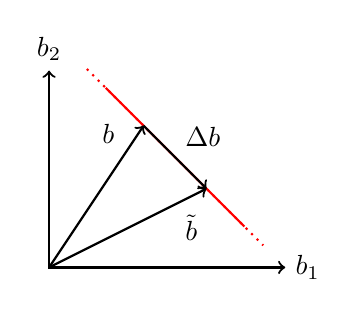
\begin{tikzpicture}
    % Draw axes
	\coordinate (borig) at (1.2,1.8);
    \coordinate (b) at (2,1);
	\coordinate (db) at ($(b)-(borig)$);

    \draw [<->,thick] (0,2.5) node (yaxis) [above] {$b_2$}
        |- (3,0) node (xaxis) [right] {$b_1$};


%Add subspace 
	\draw[thick,red,dotted] ($-0.9*(db)+(borig)$) -- ($0.9*(db)+(b)$);
	\draw[thick,red] ($-0.6*(db)+(borig)$) -- ($0.6*(db)+(b)$);
	
	\draw[thick,->] (borig) -- node[anchor=south west ,pos = 0.5] {$\Delta b$} (b);
	\draw[thick,->] (0,0) -- node[anchor=south east,pos = 0.8] {$b$} (borig);
    \draw[thick,->] (0,0) -- node[anchor=north west,pos = 0.8] {$\tilde{b}$} (b);

\end{tikzpicture}
        \caption{Free adaptation}
        \label{fig:b_direct}
    \end{subfigure}
    \begin{subfigure}[b]{0.45\textwidth}
        \centering
        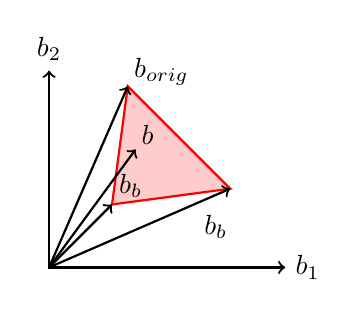
\begin{tikzpicture}
    % Draw axes
	\coordinate (borig) at (1,2.3);
    \coordinate (b_a) at (0.8,0.8);
	\coordinate (b_b) at (2.3,1);
	\coordinate (b) at (1.1,1.5);


    \draw [<->,thick] (0,2.5) node (yaxis) [above] {$b_2$}
        |- (3,0) node (xaxis) [right] {$b_1$};

    \draw[thick,red,fill = red!20] (borig) -- (b_a) -- (b_b) -- cycle;

	\draw[thick,->] (0,0) -- node[anchor=south west,pos = 0.95] {$b_{orig}$} (borig);
    \draw[thick,->] (0,0) -- node[anchor=south west,pos = 0.95] {$b_b$} (b_a);
    \draw[thick,->] (0,0) -- node[anchor=south west,pos = 0.95] {$b$} (b);
	\draw[thick,->] (0,0) -- node[anchor=north west,pos = 0.8,fill=white] {$b_b$} (b_b);

\end{tikzpicture}
        \caption{Convex adaptation}
        \label{fig:b_convex}
    \end{subfigure}
    \caption{Graphical representation of the two different approaches to adapt the weights for
    a two-stage method.}\label{fig:b_space}
\end{figure}


\subsection{Adaption of the timestep using the dense output formula}

{\bf Need to also discuss relaxing the order conditions}

If the original step $\dt$ was too large and there is no suitable set of weights, the LP is infeasible. In this case we would like to calculate $u^{n+\theta}$ using the stage values instead of rejecting the step. The time step is reduced after computing the stage values. This can be done using the order conditions for dense output \cite[Section~II.6]{hairer_solving_1993}.
We introduce $\theta \in (0,1]$. The new step taken has the length $\theta \dt$, where $\dt$ is the time step used when calculating the stage values.
To calculate a reduced step the order conditions have to be adapted and a new $b(\theta)$ for the objective function has to be generated. 
When adapting the order condition to a new $\theta$ the order condition matrix $Q$ stays unchanged whereas the right hand side $r(\theta)$ depends on $\theta$.

The dependency of $r(\theta)$ is nonlinear. This means that the maximum $\theta$ with suitable weights cannot be calculated by solving a LP. This means that different $\theta$ have to be tested. 
%(Note: we could include some algorithm to search for it)

\subsubsection{Construction of embedded methods}

As a first order method, the weights that correspond to a series of backward Euler steps are added. These are known to yield a positive result for any step size.
It is also possible to add embedded methods of higher order.
An important property of the embedded methods is that they should show the desired stability characteristics. 

A reduction of the step size using the order conditions for dense output would also be possible. For this a set of embedded methods $b_1(\theta),\cdots,b_d(\theta)$ has to be constructed. This was not the aim of this research.

(Note: Doing dense Output here is a bit complicated, but it would not help ensure positivity only (maybe) increase exactness.  is it worth exploring this or is it better to just leave this open for further research it may be also interesting regardless the study of positivity)

\todo{TODO} Is this approach used in the numerical experiments?
If not, we could/should probably remove this part%TODO

 
\section{Properties of adaptive RKM} \label{sec:integration}

In the previous sections an algorithm for choosing positivity preserving weights $\tilde{b}$ has been presented.
Here, we explain how this algorithm can be integrated into the framework of existing solvers.

\subsection{Choice of baseline method}
An important property of the baseline method is the existence of embedded methods and the degrees of freedom for the weights $b$.
As noted in Section~\ref{sec:OrderCond} the number of stages has to be higher than the order.
Therefore, explicit RKMs are interesting, because an explicit RKM of order $p$ requires at least $p$ stages.
Fully implicit RKMs can achieve higher orders.
To fulfill $p<s$ the order has to be reduced drastically. Therefore, these methods are not good candidates for the adaptation. 
As stated in \cite{norsett_attainable_1977} the highest achievable order of a diagonally implicit RKM is $s+1$. This condition is far closer to the condition required for the adaptation.
Another important property is the number of degrees of freedom for the choice of the new weights.  
These can be calculated using $s-\mathrm{rank}(Q)$. %$\mathrm{dim}(\mathrm{ker}(Q))$. 
The number of degrees of freedom for different explicit methods are shown in Table\,\ref{table:DOF_exp}.
 
\begin{table}[h!]
\centering    %Generated below============ 
% \begin{tabular}{|l c|c c c c c c |}
%  \hline
% Order & &1&2&3&4&5&6 \\
%  \hline Classical RK4& s=4&3&2&0&0& - & -  \\
%  SSPRK(10,4)& s=10&9&8&6&4& - & -  \\
%  Cash-Karp RK5(4)6& s=6&5&4&2&1&0& -  \\
%  Dormand-Prince RK5(4)7& s=7&6&5&3&1&0& -  \\
%  \hline
%  \end{tabular}
  \begin{tabular*}{\linewidth}{@{\extracolsep{\fill}}lr*6c@{}}
    \toprule
    Method & $s$ & \multicolumn{6}{c}{Order $\tilde p$} \\
    & & 1 & 2 & 3 & 4 & 5 & 6 \\
    \midrule
    Classical RK4 \cite{kutta1901beitrag} & 4 & 3 & 2 & 0 & 0 & --- & --- \\
    SSPRK(10,4) \cite{ketcheson2008highly} & 10&9&8&6&4& --- & ---\\
    Cash--Karp RK5(4)6 \cite{cash1990variable} & 6&5&4&2&1&0& --- \\
    Dormand--Prince RK5(4)7 \cite{prince1981high}& 7&6&5&3&1&0& --- \\
    \bottomrule
  \end{tabular*}
  \caption{Degrees of freedom for the choice of the weights for some explicit methods.} %Generated above============
  \label{table:DOF_exp}
\end{table}
 
\begin{table}[h!]
\centering   %Generated below============ 
%   \begin{tabular}{|l c|c c c c c c |}
%   \hline
%   Order & &1&2&3&4&5&6 \\
%   \hline Implicit Euler& s=1&0& - & - & - & - & -  \\
%   Lobatto~IIIC4& s=4&3&2&1&0&0&0 \\
%   Radau~IIA3& s=3&2&1&0&0&0& -  \\
%   SDIRK(5,4)& s=5&4&3&1&0& - & -  \\
%   TR-BDF2& s=3&2&1& - & - & - & -  \\
%   Im-Euler 2& s=3&2&1& - & - & - & -  \\
%   Im-Euler~3& s=6&5&4&2& - & - & -  \\
%   Im-Euler 4& s=10&9&8&6&3& - & -  \\
%   \hline
%   \end{tabular}
   \begin{tabular*}{\linewidth}{@{\extracolsep{\fill}}lr*6c@{}}
    \toprule
    Method & $s$ & \multicolumn{6}{c}{Order $\tilde p$} \\
    & & 1 & 2 & 3 & 4 & 5 & 6 \\
    \midrule
    Implicit Euler& 1&0& --- & --- & --- & --- & ---  \\
    Lobatto~IIIC4 \cite{chipman1971stable} & 4&3&2&1&0&0&0 \\
    Radau~IIA3 \cite{ehle1969pade} & 3&2&1&0&0&0& ---  \\
    SDIRK(5,4) \cite[eq. (6.18)]{hairer_solving_1996}& 5&4&3&1&0& --- & ---  \\
    TR-BDF2 \cite{bank1985transient} & 3&2&1& --- & --- & --- & ---  \\
    Extrapolation Im-Euler 2& 3&2&1& --- & --- & --- & ---  \\
    Extrapolation Im-Euler~3& 6&5&4&2& --- & --- & ---  \\
    Extrapolation Im-Euler 4& 10&9&8&6&3& --- & ---  \\
    \bottomrule
  \end{tabular*}
  \caption{Degrees of freedom for the choice of the weights for some implicit methods.} %Generated above============
  \label{table:DOF_imp}
\end{table}


For all methods with the number of stages equal to the order of the method, there are no degrees of freedom without reducing the order.  
If the classical RK4 method is used the order has to be reduced more because the RK4 method does not have embedded methods of order~3.
In contrast to this, methods with $s > p$ have degrees of freedom even without reducing the order.
For Cash--Karp RK5 and Dormand--Prince RK5 the order has to be reduced to get degrees of freedom even though the number of stages is higher than the order.


In Table\,\ref{table:DOF_imp}, the same properties of some implicit
methods are reported.
We can see that the fully implicit methods Lobatto~IIIC4 and Radau~IIA3 require a drastic reduction of the order as expected.
The diagonally implicit SDIRK(5,4) method only requires an order reduction of one to get one degree of freedom for the weights.
The TR-BDF2 method even allows adaptations without reducing the order.  
The implicit Euler extrapolation methods also exhibit degrees of freedom without a reduction of the order.

Another important property is the stability region. 
The adaption of the weights does not solve issues with stability when used with a too big $\dt$. Therefore, the RK method has to be stable for large $\dt$.

%(Note: up to this point I do not understand why some methods perform better than other. We only see it occur depending on the Problem-RKM combination) 

A third property is the existence of a positive solution. This corresponds to the question whether there is an embedded first order method that ensures positivity. This is particularly interesting for implicit methods, because $\dt$ can be unrestricted by stability requirements.
If we have an embedded first order method, we can ensure that there is always a positive solution, which might be of first order.
This is the case for the Im-Euler extrapolation methods, because they contain a chain of BE steps. 
For explicit methods the FE method is always embedded, but a reduction of the step size might be required. 

\subsection{Error detection and approximation}
When changing the weights the solution $u^{n+1}$ is changed. 
By incorporating the order conditions for a certain order the space of possible weights that can be chosen is limited to an affine subspace.
Now it is important to know if the new solution $u^{n+1}$ still resembles the solution of the ODE $u(t_{n+1})$. 
This can be seen in the example in Section~\ref{sec:example_lin}.
This gives rise to the question whether the new solution is reasonable.
This also poses the problem on developing a system that can decide whether the new solution is acceptable or has to be rejected.


For this approach it is difficult to give some mathematically rigorous statement regarding the convergence of the method, because it only applies if the error of the original method causes the solution to get negative. This can only happen if the truncation error is large enough. This requires $\dt \gg 0$ where lower coefficients of the Taylor series are no longer sufficient to approximate the behavior. 
One could say that the main idea of the adaption of the weights alters the error in a certain way, so that the numerical solution gets 'better' in the sense that it leads to positive solutions. 
The local error of an RKM $e(\dt) =u(t_0 + \dt) - u^1$ can be expressed using the Taylor series of the RKM and the Taylor series of the exact solution, % Hairer I P134
\begin{align}\label{eq:Taylor_sol_ref}
u(t_0 + \dt) &= u(t_0) + u'(t_0) \dt + \frac{u''(t_0)}{2} \dt^2 + \cdots + \frac{u^{(p)}(t_0)}{p!} \dt^p + \frac{u^{(p+1)}(t_0)}{(p+1)!} \dt^{p+1} + \cdots, \\
u^{n+1} &= u(t_0)  + v_1 \dt + \frac{v_2}{2} \dt^2 + \cdots + \frac{v_p}{p!} \dt^p + \frac{v_{p+1}}{(p+1)!} \dt^{p+1} + \cdots .
\end{align}
The derivatives of $u(t)$ can be solely expressed with the partial derivatives of the RHS $f(t,u)$, whereas the coefficients $v_1,v_2,\cdots$ also depend on the RKM. 
In this case the RKM is fixed apart from the weights. 
Therefore $v_1,v_2,\cdots$ are functions of $b$.
Because the weights are chosen to ensure the order conditions, the coefficients $v_1,\cdots,v_p$ are fixed and equal the according derivatives.
The only remaining degrees of freedom are the coefficients $v_{p+1},v_{p+2},\cdots$.
These can be adapted by changing the weights.

%The main way to ensure that the RKM with adapted b converges to the correct solution is to ensure that the weights approaches $b_{orig}$ for $\dt \to 0$. For this the weights it is already known that the numeric solution converges to the exact solution.  
%This is made sure by the property of the Objective function that 
%\begin{equation}
%\mathrm{argmin}(f_{optim}(b)) = b_{orig}
%\end{equation}
This approximation is not very useful for real applications. 
To approximate the error of a new step we propose the following approximation of the local error:

\begin{align}
err = |u(t^{n+1})-u^{n+1}| &= |u(t^{n+1}) - (u^{n+1}_{unadapted}+\dt F(\tilde{b}-b))| \\
 &\leq \underbrace{|u(t^{n+1})-u^{n+1}_{unadapted}|}_{\approx err_T}+\underbrace{|\dt F(\tilde{b}-b)|}_{= err_{adapt}} \label{eq:Err}
\end{align}

The total error is split up in the truncation error $err_T$ and the adaption error $err_{adapt}$ using the triangle inequality. 
The truncation error can be estimated using the standard error estimators $err_T = | u^{n}_{b_{orig}} - u^{n}_{\hat{b}} |$. 
After adapting the weights, the adaption error is calculated. If the adaption error is larger than the tolerance the weights are rejected.
Both errors are added to get an approximation of the total error $err = err_T + err_{adapt}$.
% The truncation error and the adaption error never have the same direction.
% Therefore, the triangle inequality becomes a strict inequality and the real error is always smaller than the estimate. (Note: as long as the Truncation error estimator is right)
%\subsubsection{Steppsize Control}
%An important part of an RKM method is the ability to approximate the error of the solution to use it to control the step size. 
%The truncation error $|u(t^n)-u^n_{b_{orig}}|$ is usually approximated with an standard error estimator $err_T = | u^{n}_{b_{orig}} - u^{n}_{\hat{b}} |$.
 %The parameter $w_a \leq 1$ is used to account for the fact that the real error is smaller than $err = err_T +err_{adapt}$. The factor also improves the stability of the step size control because $err_{adapt}$ is not as smooth as $err_T$, especially if negative values only occur for a small number of steps.
%If the LP was infeasible and no weights were found the $err_{approx}$ is set to a custom value. This value should be chosen sufficiently large to ensure that the next step take is smaller, but still not too large to keep the step size control stable.
This type of error estimation is easy to implement because it can be easily incorporated in an existing step size control and takes advantage of the standard error approximation.

%To make sure that the new adapted solution is still reasonable we measure the deviation from the Original method. In the worst case the errors add up. (todo: here some math formula... (We know that cannot be the case because we already know that we will reduce the error for the quantity we will make positive, still we can use it as a upper bound.))

\subsection{Stability region}

Adapting the weights $b$ changes the RK method. Hence, the stability
function is altered and the region of absolute stability varies.
How often and how much the stability function is changed depends
of course on the problem, the RKM, and the timestep $\dt$.
For problems where only a small number of steps are affected, a bigger
change in the stability function might be acceptable. For problems
that require an adaptation of the weights for every step, one needs
to make sure that the resulting method is stable.

The stability regions of adapted RKMs are visualized in
Figure\,\ref{fig:stab}.
In Figure\,\ref{fig:stab_dp5} the Dormand--Prince RK5 method is freely adapted.
The weights are taken from the example in Section~\ref{sec:Ex_expl}.
In Figure\,\ref{fig:stab_ex3} the stability regions of the Im-Euler~3
extrapolation method and the embedded chain of three BE steps are
plotted. Additionally the stability regions of convex combinations
of these two methods are shown.

\begin{figure}
     \centering
     \begin{subfigure}[b]{0.45\textwidth}
         \centering
         \includegraphics[width=\textwidth]{plots/stab_dp5.pdf}
         \caption{Dormand--Prince RK5 with free adaptation
                   of the weights $\bt$ as in the example in Figure~\ref{fig:weights_AdDe}.}
         \label{fig:stab_dp5}
     \end{subfigure}
     \hfill
     \begin{subfigure}[b]{0.45\textwidth}
         \centering
         \includegraphics[width=\textwidth]{plots/stab_ex3.pdf}
         \caption{Im-Euler~3 extrapolation method and embedded chain
                  of three BE steps with convex combinations of both
                  weights.}
         \label{fig:stab_ex3}
     \end{subfigure}
        \caption{Change of stability region for the free adaptation and
                 the convex adaptation of the weights.}
        \label{fig:stab}
\end{figure}


The stability function is defined as a function $\CN \to \CN$ with
\begin{equation}
R(z) = 1 + zb^T(I - zA)^{-1}e,
\end{equation}
where $e = (1, \dots, 1)^T \in \R^s$.
We can add $b$ as a second parameter and get a function
$R\colon \R^s \times \CN  \to \CN$ with
\begin{equation}
R_b(z) = 1 + zb^T(I - zA)^{-1}e.
\end{equation}
The stability function is an affine-linear function of the weights.

%TODO: It is not straightforward if there are no pole zero cancellations in the stability function. For explicit methods, the stability function is a polynomial o degree $\leq s$ (Hundsdorfer). Pole zero cancellations cannot happen for these. For implicit functions that are A-stable the poles have to be in the right halve plane. Here is starts to get interesting. Because the A-Stability of one method with a certain $A$ is not a sufficient condition that there are no Poles for all RKM with this A-Matrix. But it is possible (or easy) to prove that if $a_{ii} > 0 \forall i = 1,\cdots , s$ then there are only poles in the right halve plane where they do not matter for the further considerations.)


\subsubsection{Stability of convex adaptation}

If the new weights are chosen by convex adaptation of given weights,
it is easy to prove some properties of the stability region.
\begin{theorem}
  The stability region of a Runge--Kutta method $(A,b)$ where
  $b = \sum_{i} g_i b^i$ is a convex combination of
  $b^1, \dots, b^m \in \R^s$ (i.e.\ $g_i \in [0,1]$, $\sum_i g_i = 1$),
  contains at least the intersection of the stability regions of
  the methods $(A,b^1), \dots, (A,b^m)$.
\end{theorem}
\begin{proof}
  Since the stability function is an affine-linear function of the
  weights, $R_{\sum_i g_i b^i}(z) = \sum_i g_i R_{b^i}(z)$. Hence,
  if $z$ is in the stability region of all methods $(A,b^1), \dots, (A,b^m)$,
  \begin{equation}
    | R_{\sum_i g_i b^i}(z) |
    \le
    \sum_i g_i | R_{b^i}(z) |
    \le
    1.
  \end{equation}
\end{proof}

This result is particularly important for implicit methods.
If all the embedded methods used to construct the new weights
are A-stable, the resulting method is also A-stable.


\subsubsection{Stability of free adaptation}
If the weights is adapted freely there is no such proof.
A useful property of the resulting stability region is that it is similar to the stability region of the baseline method. 
(Note: is it possible (or needed at all) to give some statement like: If the stability regions of the RKM used for multiple steps are similar, then the overall method is stable for the intersection of the stability regions.)

For most methods, a small change of the weights does not alter the stability function dramatically.
(TODO: I am missing a piece here from ‘the derivative is finite’ to ‘is similar’)

We would like to calculate the derivative of the border in respect to a change of the weights. 

The stability function depending on the weights is expressed. 
When adapting the weights we cannot change them independently but only in ways that comply with the order conditions.
$m$ is the number of dimensions of the kernel of the order condition $m = \mathrm{dim}\{\mathrm{Ker} (Q) \}$
The $b_1,\cdots,b_m$  are the basis vectors of $\mathrm{Ker} (Q)$. With a coordinate transformation we get the coordinate vector $\hat{b}$ with the matrix $B = [b_1,\cdots,b_m]$ and $b = B \hat{b}$.

The general stability function of all embedded RKM that satisfy the order conditions $Q$ is given by

\begin{equation}\label{eq:gen_stabilityf}
R(\hat{b},z) = 1 +  (b_{orig} +B \hat{b})^T z(I - zA)^{-1}
\end{equation}
The border is defined by the implicit function 
\begin{equation}\label{eq:border}
|R(\hat{b},u+iv)|^2 -1 = 0
\end{equation}
This function can be viewed either as $\R^m \times  \CN \rightarrow \R$ or $\R^m \times  \R^2 \rightarrow \R$.
We are only concerned with the expansion or contraction. Because of this we are only interested in the change perpendicular to the border of the stability region. 

For a point $z_0= u_0 +i v_0 $ 
with $ |R(w,z_0)|^2 -1 = 0 $ the gradient of
 $|R(w,u,v)|^2$ is calculated. 
If the gradient does not vanish at $z = z_0$ \eqref{eq:border} can be transformed in a function $\R^m \times \R \rightarrow \R$ depending on $\hat{b}$ and a single variable $a$ by setting $z = z_0 + n a$. The complex number $n$ denotes the normal vector $\vec{n} = \frac{\nabla |R(\hat{b},u,v))|^2}{\left| \nabla |R(\hat{b},u,v))|^2 \right|}$ of the border of the stability region written in complex notation. This defines the function $a(\hat{b})$ with $|R(\hat{b},z_0 + n a(\hat{b}))|^2 -1 = 0$. 
This implies that this approach is only applicable if the gradient does not vanish on the border of the stability function. This is not true in general but for the most common RKM. 
The derivative $\frac{\mathrm d}{\mathrm d \hat{b}} (a(\hat{b}))$ can be calculated using the implicit function theorem. The defining function is 
\begin{equation}\label{eq:f(w,a)}
f: \R^m \times \R \rightarrow \R,  f(\hat{b},a) = |R(\hat{b},z_0 + n a)|^2 -1
\end{equation}
If explicit methods are used this function is known to be continuously differentiable because it can be written as a polynomial of $\hat{b},u$ and $v$. This is a necessary condition for the use of the implicit function theorem.
It is also known by definition, that for the point $b = b_{orig}$ and $z = z_0$ the equation $ |R(\hat{b},z_0)|^2 -1 = 0 $ is satisfied.
For simplicity only the formulas for the derivative at the value $b = b_{orig}$ are given. This corresponds to $\hat{b} = 0$.
The wanted derivative is given by 

\begin{equation}
 \frac{\partial a}{\partial \hat{b}_j} (w) =
 - \left[ \frac{\partial f}{\partial a} (\hat{b},a(\hat{b}))  \right] ^{-1} 
   \left[ \frac{\partial f}{\partial \hat{b}_j}(\hat{b},a(\hat{b})) \right]
\end{equation}
as long as $\frac{\partial f}{\partial a} \neq 0$ on the border of the region of absolute stability. This is true in most cases as it has been discussed above.

The derivative of \eqref{eq:f(w,a)} in respect to $a$ evaluated at $\hat{b}=0$ can be calculated using the directional derivative
\begin{align*}
 \frac{\partial f}{\partial a} \Big|_{\hat{b}=0} =& 
 \frac{\partial f}{\partial a} (\hat{b},a(\hat{b})) \Big|_{\hat{b}=0} = 
 \nabla |R(\hat{b},a(\hat{b})|^2 \vec{n} \Big|_{\hat{b}=0} \\
=& \left| \nabla|R(0,z_0)|^2 \right| = \left| \nabla|R_{b_{orig}}(z_0)|^2 \right|
\end{align*} 

The derivative in respect to $\hat{b}_j$ is 
$ \frac{\partial f}{\partial \hat{b}_j}(\hat{b},a(\hat{b})) \Big|_{\hat{b}=0}$.
This simplifies to 
\begin{multline}\label{eq:derivative_to_b}
 \frac{\partial f}{\partial \hat{b}_j}(\hat{b},a(\hat{b})) \Big|_{\hat{b}=0} = 
 \frac{\partial }{\partial \hat{b}}(R(\hat{b},z)R(\hat{b},z^*)) \\
 = (B\hat{b}_j)^T (I-zA)^{-1} R_{b_{orig}}(z^*) + (B\hat{b}_j)^T (I-z^*A)^{-1} R_{b_{orig}}(z)
\end{multline}
using the fact that $z_0$ is on the border of the stability region.
The derivative $(B\hat{b})^T (I-zA)^{-1} R_{b_{orig}}(z^*) (B\hat{b})^T (I-z^*A)^{-1} R_{b_{orig}}(z)$ is known to be finite for explicit methods, because it is a polynomial and $|z_0| < \infty$
The same process can be done for all points on the border of the stability region. 
As long as $\nabla|R(\hat{b},u+iv)|^2 \neq 0 \forall \hat{b} < \epsilon  \forall z$ the derivative $\frac{\partial a}{\partial \hat{b}_j} (\hat{b})$ is finite. This means that a small change of the weights only leads to a small change of the stability region.

\todo{TODO: Some better theorem?} %TODO
\begin{lemma}
  The stability function $R_{\bt}$ of an adapted RK method
  satisfies
  \begin{equation}
    | R_{\bt}(z) |
    \le
    | R_{b}(z) |
    + \| \bt - b \|_1 \| z (\I - z A)^{-1} e \|_\infty.
  \end{equation}
\end{lemma}
\begin{proof}
  Compute
  \begin{equation}
  \begin{aligned}
    | R_{\bt}(z) |
    &\le
    | R_{b}(z) |
    + | R_{\bt}(z) - R_{b}(z) |
    =
    | R_{b}(z) |
    + | z (\bt - b) (\I - z A)^{-1} e
    \\
    &\le
    | R_{b}(z) |
    + \| \bt - b \|_1 \| z (\I - z A)^{-1} e \|_\infty.
  \end{aligned}
  \end{equation}
\end{proof}
This shows why the objective $\min \| \bt - b \|_1 \|$ is a good
choice to control the change of the region of absolute stability,
in particular for explicit methods for which
$\| z (\I - z A)^{-1} e \|_\infty$ can be bounded by a polynomial
in $|z|$.


\section{Implementation aspects of the algorithm}\label{sec:imple}

Having described the mathematical idea of our approach,
we discuss some practical implementation details of the
proposed algorithm in the following.


\subsection{Positivity}

For the further discussion, we are concerned with a system of
$m$ coupled ODEs, i.e.\ $u \in \R^m$.
Systems of ODEs with a high number of dimensions can appear when solving a PDE with the method of lines.

To ensure that the solution is positive
\begin{equation}
 u_i^{n+1} \geq 0   \quad   \forall {i \in \{1, \cdots,m \}}  
\end{equation}
has to be fulfilled. These $m$ positivity constraints of the
optimization problem can be written as
\begin{equation}
u_i^n + \dt \sum_{j=0}^s F_{i,j}  b_j \geq 0 \quad \forall {i \in \{1, \cdots,m \}}
\end{equation}

Imposing all of these constraints in the LP solver usually results
in unnecessarily many constraints. In many cases, positivity is
violated only for a subset $h \subseteq \{1, \dots, m\}$ of all
components. This reduced set of positivity constraints can be
formulated as
\begin{equation}
u_i^n + \dt \sum_{j=0}^s F_{i,j}  b_j  \geq 0 \quad \forall i \in h \subseteq \{1,\cdots,m \}.
\end{equation}
A reasonable approach is to set $h_0 = \{ i \in \{1,\cdots,m \} |  u_i^{n+1}  < 0 \}$. 
After the new weights and $u^{n+1}$ are computed using $h_0$, the algorithm has to check if the positivity of the other values $\{u_i | i \notin h_0 \subseteq \{1,\cdots,m \}\}$ is still satisfied.
If the condition is not met a new set $h_{a+1} = \{ i \in \{1,\cdots,m \}|  u_i^{n+1}  < 0 \} \cup h_{a}$ using the new $u^{n+1}$ is generated and the LP is solved again. This process is repeated until a solution is found that leads to $u^{n+1} \geq 0$. The choice of $h_{a+1}$ based on $h_{a}$ ensures that the algorithm cannot get stuck in a loop. In the worst case $h_a$ is growing very slowly until $h_a = \{1,\cdots,m \}$.
This worst case did not occur when runing the testproblems. 
%(Note: A approach on this would be to make a educated guess which indices could get a problem with positivity. A possible estimate would be $\frac{u_i^{n+1}}{max(K_{(i,0)}, \cdots ,K_{(i,0)})} $ )

When enforcing a maximum value, the number of constraints can be reduced using the same technique. When enforcing both maximum and minimum values two separate sets of active constraints $k_{min}$ and $k_{max}$ are used. The set $k_{max}$ denotes the active maximum constraints and the set $k_{min}$ denotes the active minimum constraints.
In this case it is important to update these sets simultaneously.  

\subsection{Implemention}
(\todo{TODO}: Maybe a flowchart and a description on how we stitch everything together.) %TODO

At first, the stage values $y_i$ and stage derivatives $f_i$ are calculated.
Afterwards, $u^{n+1}$ is computed using the original weights $b$.
If the positivity is not violated, this solution is used to update the solution.
If $u^{n+1}$ contains negative values, the weights are adapted using the following algorithm.

Start with the highest order $\tilde p$ such that there are degrees
of freedom for the weights $\bt$. Apply an LP solver to the optimization
problem with accuracy and positivity constraints.
If the LP is infeasible, reduce the order $\tilde p$ by one.
If the LP is feasible, test whether the solution is acceptable.
At first, test whether the new $u^{n+1}$ satisfies the constraints.
This is necessary because sometimes the applied LP solvers incorrectly
identify the problem as feasible.
Afterwards the adaption error is calculated using \eqref{eq:Err}.
If the error is bigger than a given maximum error tolerance, the
new weights $\bt$ are also rejected.
If the new set of weights is rejected in one of the tests the order
$\tilde p$ is reduced by one.
As soon as the algorithm finds suitable weights, these are used to update the solution.
If all acceptable orders are tried and no weights were found, the step hast to be rejected.

If the reduction of stepsize is used this process is done first for $\theta = 1$. If no weights were found, the process is repeated for a smaller $\theta$.



\section{Results of numerical experiments}\label{sec:Numeric_Results}

The implementation of the algorithms described above and code to
reproduce the numerical examples reported here can be found in
\cite{repository}. \todo{TODO: New reopsitory with DOI} %TODO
The methods are implemented in Python using NumPy/SciPy
\cite{virtanen2019scipy}, NodePy \cite{nodepy08}, and
Matplotlib \cite{hunter2007matplotlib} for the visualizations.
We have used CVXPY to solve the LPs \cite{cvxpy, cvxpy_rewriting}.
\todo{TODO: Which solver of CVXPY?} %TODO



\subsection{Applicable problems}\label{sec:app_problem}
The approach can be used with ODE systems $u' = f(t,u)$ that ensure  $u(t) \geq 0 \forall t \forall {  u_0 \geq 0}$ 
A sufficient condition is  
\begin{equation}
u_i=0 \implies f_i(t,u_1,\cdots,u_i,\cdots,u_n) \geq 0 \quad \forall {u_c \geq 0}\; \forall {t}
\end{equation}
For problems where the exact solution is positive for certain $u_0$ but positivity is not preserved for all $u_0 \geq 0$ tests did not show promising results. Additionaly it is not certain if the computed solutions would be reasonable.

\todo{Note (HR)} I think this should be moved to the beginning.


\subsection{Explicit methods}\label{sec:Ex_expl}
First we want to test the adaptive RKM used with explicit methods.  
When used with explicit methods the cost of solving the LP is significant because the computation of the stage derivatives only requires $s$ evaluations of the RHS.
For most of the linear test problems tried, the explicit methods yield to positive results.  
When increasing the step size, issues with stability occur before getting negative values.  
An example for this is the ODE in Section~\ref{sec:example_lin}.
Some nonlinear RHS may require very small timesteps to preserve positivity.  
For these, adapting the weights could be a possible way to solve them. 
An example is the reaction equation solved in Section~\ref{sec:example_reac}.
Since the positivity of the stage values is not ensured, the right hand side has to be defined for negative values. If this is not the case, the right hand side has to be adapted accordingly.

A test problem similar to \cite{shampine_non-negative_2005} is the PDE
\begin{equation}
\begin{aligned}
  \frac{\partial u(t,x)}{\partial t}
  &=
  -a \frac{\partial u(t,x)}{\partial x} - K u(t,x),
  && x \in (0, 1), t \in (0,1),
  \\
  u(t,0) &= 1,
  && t \in (0,1],
  \\
  u(0,x) &= 0,
  && x \in [0,1],
\end{aligned}
\end{equation}
which consists of an advection part and an exponential decay.
The numerical approximation uses the method of lines and a first order
upwind finite difference semidiscretization with $N = 100$ points.
This leads to the positivity preserving ODE
\begin{equation}
\frac{\mathrm d}{\mathrm d t} u_i = \frac{a}{\Delta x} \left( u_{i-1} - u_i \right) - K u_{i-1}.
\end{equation}
The parameters are set to $a=1$ and $K=1$.
We use the Dormand--Prince RK5 method and adapt the weights using the free adaptation.
In Figure\,\ref{fig:sol_AdDe} the results for $\Delta t = 0.02$ are plotted for different timesteps. We can see that the solution approaches an exponential function with $t \rightarrow \infty$.
In Figure\,\ref{fig:weights_AdDe} the used weights are plotted. For $t\leq 0.6$ the weights are altered. For $t > 0.6$ the original weights lead to a positive solution.
\begin{figure}
\centering
\begin{subfigure}[t]{0.45\textwidth}
\centering
\includegraphics[width=1\textwidth]{plots/Advection_Decay.pdf}
\caption{Numerical solution at different times.}
\label{fig:sol_AdDe}
\end{subfigure}%
~
\begin{subfigure}[t]{0.45\textwidth}
\centering
\includegraphics[width=1\textwidth]{plots/b_Advection_Decay.pdf}\\
\caption{Adaptation of the weights.}
\label{fig:weights_AdDe}
\end{subfigure}
\caption{Numerical results for the advection decay problem.}
\end{figure}


Next, different timesteps are used.
For $\dt \leq 0.0082$ the unaltered method leads to positive solutions. For a larger $\dt$ the original method leads to negative values and the weights are altered. For $\dt >0.016$ the baseline method is no longer stable.
For the ODE, the reference solution can be computed using the matrix exponential. 
In Figure\,\ref{fig:conv_expl} the convergence for $t=0.5$ is plotted for the altered and unaltered method.

\begin{figure}[ht]
\centering
\includegraphics[scale=0.6]{plots/conv_adde.pdf}
\caption{Convergence results of the adapted Dormand--Prince RK5.}
\label{fig:conv_expl}
\end{figure}

The unaltered method has the order $p=5$. 
The values marked with a cross denote the numerical experiments that required an adaption of the weights. 
Even though the order is reduced, most errors are still close to the error of the unaltered method.

\subsection{Implicit methods}
Implicit methods seem like an advantageous choice for a couple of reasons. 
Firstly, the cost of solving the LP is relatively small compared to the cost of solving the stage equations.
Secondly, the timestep is not limited by the stability of the method.
Therefore, it is possible to use larger timesteps that are more likely to lead to negative values.

A very interesting class of methods are the implicit extrapolation methods. These are diagonally implicit and $p < s$. This means that they allow for changes of the weights without a reduction of the order.
Also, all stage values are computed using the BE method. Hence, all intermediate stages are positive.
Also, an embedded BE step is included. This ensures that a positive solution always exists, even if it is of first order.

We test the proposed adaptation algorithm on the diffusion equation
\begin{equation}
\frac{\partial }{\partial t} u = D \frac{\partial^2}{\partial x^2} u
\end{equation}
with homogeneous Dirichlet boundary conditions on the domain $x = [-0.5,0.5]$ with $N=100$ points. The equation is semidiscretized using the 3-point-scheme
\begin{equation}
\frac{\mathrm d}{\mathrm d t} u_i = \frac{d}{\Delta x^2} \left( u_{i-1} - 2u_i + u_{i+1} \right)
\end{equation}
As initial condition $u^0 = (0,\cdots,0,1,0,\cdots,0)^T$ is used. The diffusion coefficient is $D=1$.

The ODE is solved using the Im-Euler~3 extrapolation method.
For large $\dt$ the method computes negative values for $u^1$.
These can be corrected by adapting the weights.  
The solutions are computed using the free adaptation and convex adaptation for $\dt = \num{1e-3}$.
The results for the free adaptation are plotted in Figure\,\ref{fig:sol_Diff_a} and the corresponding change of the weights
is shown in Figure\,\ref{fig:weights_Diff_a}.
The original solution for the first step is negative. Therefore, the weights have to be changed. 
If we take a look at the solution after the first timestep at $t=0.001$ we can see that at $x=0$ the solution is smaller than the solution at the surrounding points.  
This is not physical.  
The next timesteps lead to physical solutions again. 
To prevent this glitch from happening we choose the weights based on a convex adaptation. 
A first order embedded method is added. The solution is shown in Figure\,\ref{fig:sol_Diff_c} and the weights are visualized in Figure\,\ref{fig:weights_Diff_c}.
The weights for the first step are altered again. 
The weights obtained by the convex adaptation are different from the weights obtained 
by taking the free adaptation. 
The solution for $t=0.001$ computed with the convex adaptation is physical. 
For both approaches, the remaining steps can be computed with the standard weights. 
\begin{figure}
\centering
\begin{subfigure}[b]{0.45\textwidth}
\centering
\includegraphics[width=1\textwidth]{plots/Diff_Direct.pdf}
\caption{Solution using the free adaptation.}
\label{fig:sol_Diff_a}
\end{subfigure}
\begin{subfigure}[b]{0.45\textwidth}
\centering
\includegraphics[width=1\textwidth]{plots/Diff_Convex.pdf}
\caption{Solution using the convex adaptation.}
\label{fig:sol_Diff_c}
\end{subfigure}
\\
\begin{subfigure}[b]{0.45\textwidth}
\centering
\includegraphics[width=1\textwidth]{plots/b_Diff_Direct.pdf}
\caption{Change of weights for free adaptation.}
\label{fig:weights_Diff_a}
\end{subfigure}
\begin{subfigure}[b]{0.45\textwidth}
\centering
\includegraphics[width=1\textwidth]{plots/b_Diff_Convex.pdf}
\caption{Change of weights for convex adaptation.}
\label{fig:weights_Diff_c}
\end{subfigure}
\caption{Numerical results for the diffusion problem and the
         adapted Im-Euler~3 extrapolation method.}
\end{figure}


In Figure\,\ref{fig:conv_impl}, the convergence is shown for the unaltered Im-Euler~3 extrapolation method (ex3, potentially resulting in negative values), the adaptive method with free adaptation (ex3a) and the adapted method using convex adaptations (ex3c).
Also, the BE method is plotted. It is only of 1st order but preserves positivity for all $\dt$. 
For $\dt < \num{3e-5} $ the standard weights yield to a positive result. For larger $\dt$ the weights have to be adapted to ensure positivity. 
The ex3a shows similar convergence properties as the original method.
This can be expected, because the adapted method is still of 3rd order. 
The ex3c has larger errors than the ex3a but leads to physical solutions for all time-steps.
This is no surprise because the adapted RKM used for the first step is only of first order.
But the adaptive method still outperforms the BE, even when accounting for the higher cost per step. 

\begin{figure}[ht]
\centering
\includegraphics[scale=0.75]{plots/conv_heat.pdf}
\caption{Convergence result of baseline and adapted Im-Euler~3
         extrapolation methods for the diffusion problem.}
\label{fig:conv_impl}
\end{figure}


\subsection{Stepsize control}

Next we test the adaptive RKM on a more complex problem. 
For this, we consider the advection-diffusion-production-destruction systems from \cite{kopecz_comparison_2019}. The system is defined by
\begin{subequations}
\label{eq:ADR}
\begin{align}
\frac{\partial u_1}{\partial t} &=-a \frac{\partial u_1}{\partial x} + d\frac{\partial^2 u_1}{\partial x ^2} + 0.01u_2 + 0.01 u_3 +0.003u_4 - \frac{u_1 u_2}{0.01+u_1} \\ 
\frac{\partial u_2}{\partial t} &=-a \frac{\partial u_2}{\partial x} + d\frac{\partial^2 u_2}{\partial x ^2} + \frac{u_1u_2}{0.01+u_1} -0.01 u_2-0.5(1-\exp(-1.21 u_2^2)) u_3 -0.05 u_2 \\ 
\frac{\partial u_3}{\partial t} &=-a \frac{\partial u_3}{\partial x} + d\frac{\partial^2 u_3}{\partial x ^2} + 0.5(1-\exp(-1.21u_2^2)) u_3 - 0.01 u_3 -0.02 u_3 \\ 
\frac{\partial u_4}{\partial t} &=-a \frac{\partial u_4}{\partial x} + d\frac{\partial^2 u_4}{\partial x ^2} + 0.05 u_2 + 0.02 u_3 + 0.003u_4 
\end{align}
\end{subequations}
with parameters $a=\num{1e-2} $ and $ d=\num{1e-6}$.
The PDE is simulated on the domain $x = [0,1]$ with $N=100$ points. Periodic boundary conditions are used. 
The advection part is semidiscretized using a first order upwind scheme and the diffusion part is semidiscretized using a 3-point-scheme. This leads to a positivity preserving system of ODEs.
The computation is done using the Im-Euler~3 extrapolation
method with free adaptation.
As step size control a PI-control from\,\cite{hairer_solving_1996} is used. The error was estimated using \eqref{eq:Err}. The tolerance was set to $Tol = 0.01$.
The final time is $t_{end} = 50$.

The simulation required 264 steps. Of these, 72 required an adaptation of the weights. 
All adapted weights are still of 3rd order.
The solutions for $t=9,t=18,t=27$ and $t=50$ are plotted in Figure\,\ref{fig:Sol_ADP}. 
In Figure\,\ref{fig:sol_ADP18} it can be seen that the reaction occurs in a small interfaces. 
Outside of this regions quantities are close to zero. Therefore, it is very likely that negative values occur in the numerical approximation.
In Figure\,\ref{fig:sol_ADP27} it can be seen that at $T=27$ the two reaction interfaces merged. Afterwards the reaction stops and the behavior is mainly controlled by the advection and diffusion part.  

In Figure\,\ref{fig:Stats_ADP} different values are plotted.  
In the first subplot the step size is plotted. For $t<25$ the timesteps are small. After $t = 30$ the step size increases, because the solution only evolves slowly afterwards. 
In the second subplot the minimum of $u_1,u_2,u_3,u_4$ is plotted for all timesteps that initially lead to negative values. This value is computed before and after adapting the weights.
We can see that relatively large negative values occurred at some timesteps. 
After the adaption of the weights, all values are close to $0$. Therefore, the adaption of weights successfully preserved positivity. 
In the third subplot the approximated truncation error $err_T$ and the adaption errro $err_{adapt}$ are plotted. 
We can see that the adaption error is of a similar magnitude as the truncation error. Therefore, the total error of the method is not increased drastically.  
In the last subplots the weights are plotted.  
We can see that the changes to the weights are only very small. The adapted RKM is still very close to the original RKM. 

\begin{figure}
    \centering
    \begin{subfigure}[b]{0.49\textwidth}
        \includegraphics[width=\textwidth]{plots/ADP_sol_00.pdf}
        \caption{$t=0$.}
        \label{fig:sol_ADP00}
    \end{subfigure}
    \begin{subfigure}[b]{0.49\textwidth}
        \includegraphics[width=\textwidth]{plots/ADP_sol_18.pdf}
        \caption{$t=18$.}
        \label{fig:sol_ADP18}
    \end{subfigure}
    
    \begin{subfigure}[b]{0.49\textwidth}
        \includegraphics[width=\textwidth]{plots/ADP_sol_27.pdf}
        \caption{$t=27$.}
        \label{fig:sol_ADP27}
    \end{subfigure}
	\begin{subfigure}[b]{0.49\textwidth}
        \includegraphics[width=\textwidth]{plots/ADP_sol_50.pdf}
        \caption{$t=50$.}
        \label{fig:sol_ADP50}
    \end{subfigure}
    \caption{Solution of advection-diffusion-reaction problem at different times.}\label{fig:Sol_ADP}
\end{figure}

\begin{figure}
\centering
\includegraphics[width=0.85\textwidth]{plots/ADP_stepsize,b.pdf}
\caption{Different statistics of computation of the advection-diffusion-reaction problem.}
\label{fig:Stats_ADP}
\end{figure}

\todo{Note (HR)} Should the minimum of $u$ in Figure~\ref{fig:Stats_ADP} be negative before the adaptation? %TODO


\section{Conclusion} \label{sec:conclusion}
It is possible to adapt the weights to enforce positivity for RKMs that are not positivity preserving. 
One main limitation is that the resulting order has to be lower than the number of stages.
An error approximation for this method was given.  
The region of absolute stability is altered by changing the weights. This effect can be predicted or controlled. 
Used with explicit methods the positivity for some test problems could be recovered.  
Because the time step size is limited by the stability it is only useful for a small interval of time steps. 
The adaptive method is mainly interesting for diagonally implicit methods.
The times step size is not limited by stability. 
Also, the cost of solving the LP is not a crucial factor.  
If the negative values occurring are not too large, which can be expected for most computations, adapting the weights is a potential way to ensure positivity. 

%also if exactnes is not the limiting factor but positivity 



\printbibliography

\end{document}
